\tikzsetnextfilename{spherical_harmonics}
\begin{frame}[label=local_sym_sh]{Local symmetry and spherical harmonics}
	\begin{columns}
	\column{0.25\textwidth}
	\begin{center}
	\includegraphics[width=\columnwidth]{fig_espci/hexagons}
	\end{center}
	\column{0.75\textwidth}
	\begin{tikzpicture}
		\matrix (mat) [%
			matrix of nodes, ampersand replacement=\&, nodes={anchor=center},%
			row 1/.style={font=\tiny}, row 4/.style={font=\tiny}
			]
		{
			$\ell=6, m=0$ \& \& $\ell=6, m=5$ \& \& Icosahedron\\
			
\includegraphics[width=0.25\columnwidth]{sh6-0} \& %
			$+$ \& %
			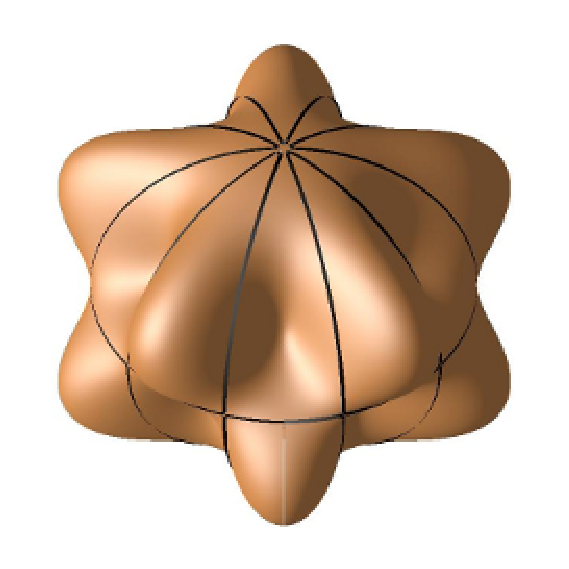
\includegraphics[width=0.25\columnwidth]{sh6-5} \& %
			$=$ \& %
			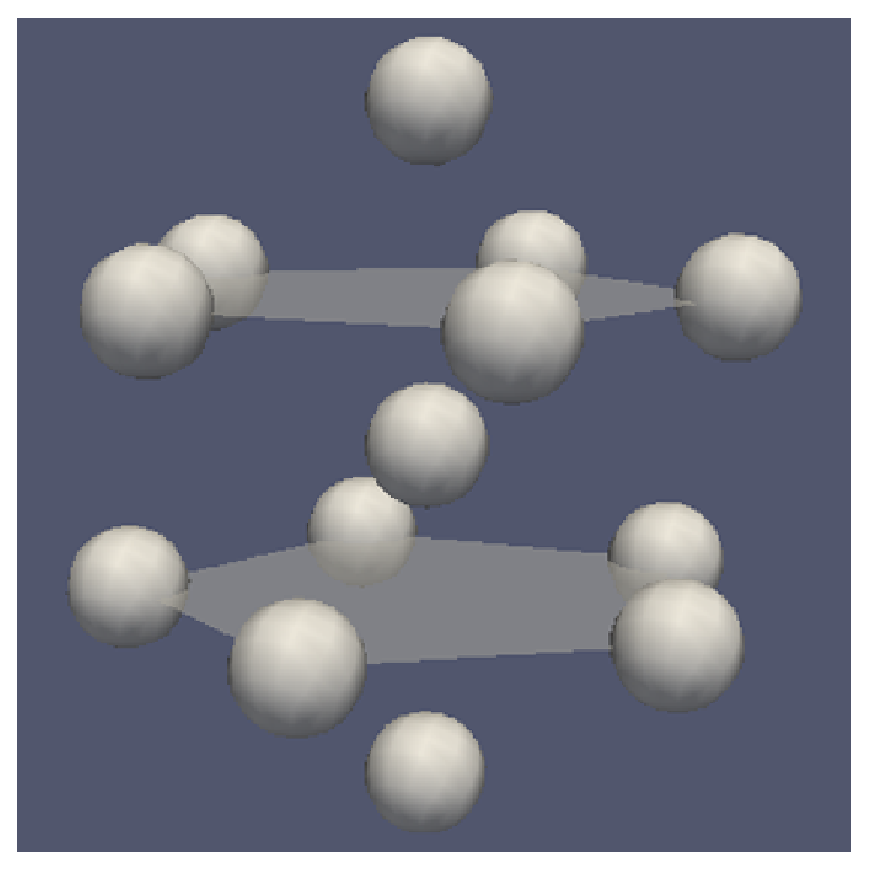
\includegraphics[width=0.25\columnwidth]{ico_13} \\
			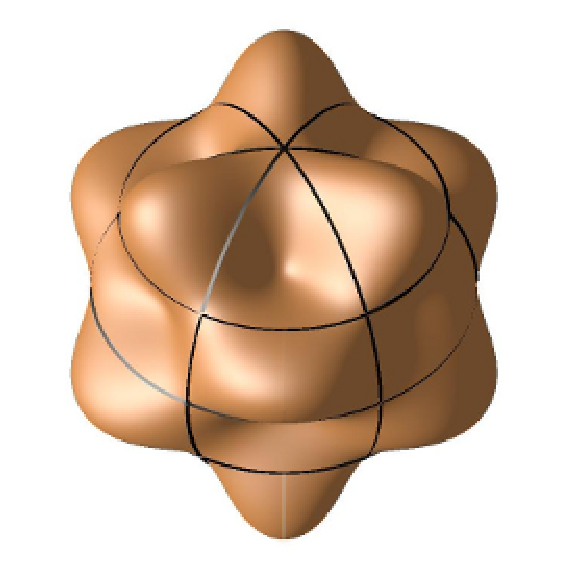
\includegraphics[width=0.25\columnwidth]{sh6-3} \& %
			$+$ \& %
			
\includegraphics[width=0.25\columnwidth]{sh6-6} \& %
			$=$ \& %
			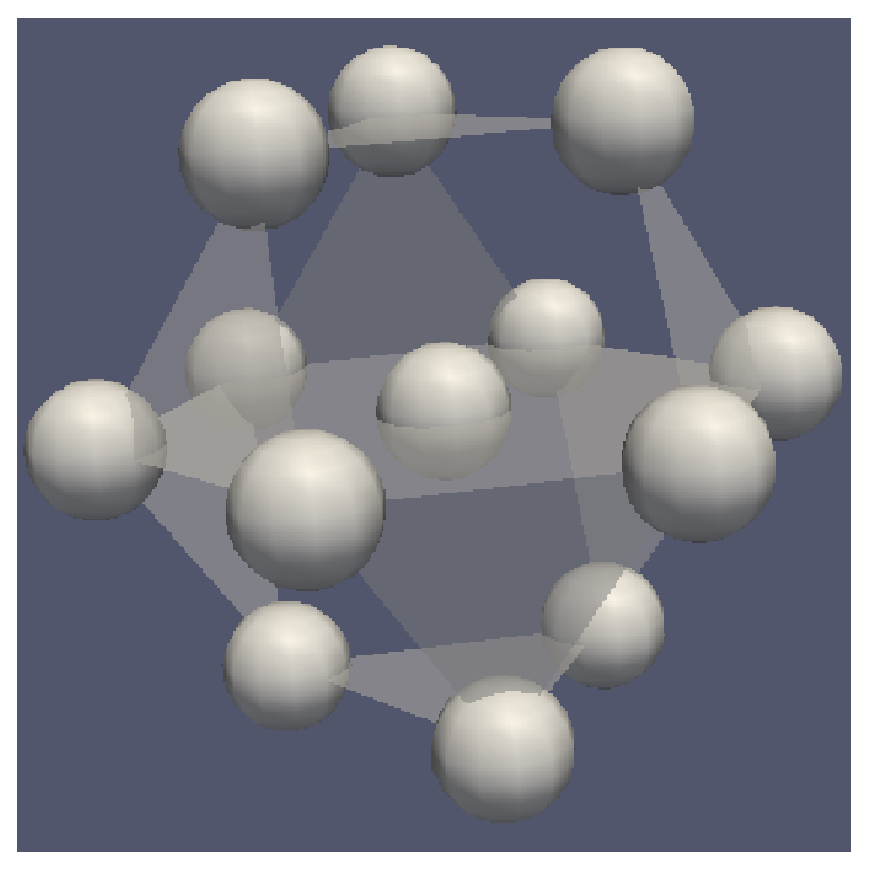
\includegraphics[width=0.25\columnwidth]{fcc_13} \\
			$\ell=6, m=3$ \& \& $\ell=6, m=6$ \& \& \textsc{fcc}\\
		};
	\end{tikzpicture}
	\end{columns}
	\begin{itemize}
		\item The orientation changes $\Rightarrow$ No positional order
		\item The local angles stay the same $\Rightarrow$ Bond orientational order
	\end{itemize}
	{\footnotesize\citet{steinhardt1983boo}}
\end{frame}


\begin{frame}<1-3>{Second-shell bond orientational order}
	\begin{textblock*}{0.6\textwidth}(10mm,88mm)
		\only<2->{\simplephasediagram{%
			\node<2-> at (0.576,0) [xp marker, fill=green!50!black] {};%
			\node<3-> at (0.497,0) [xp marker, fill=green!50!black] {};
			}}%
	\end{textblock*}
	\begin{columns}[b]
	\column{0.5\textwidth}
	\alt<-2>{\tikzsetnextfilename{Q4Q6_maps}}{\tikzsetnextfilename{Q4Q6phi3954}}%
	\begin{tikzpicture}
		\node (bcc) {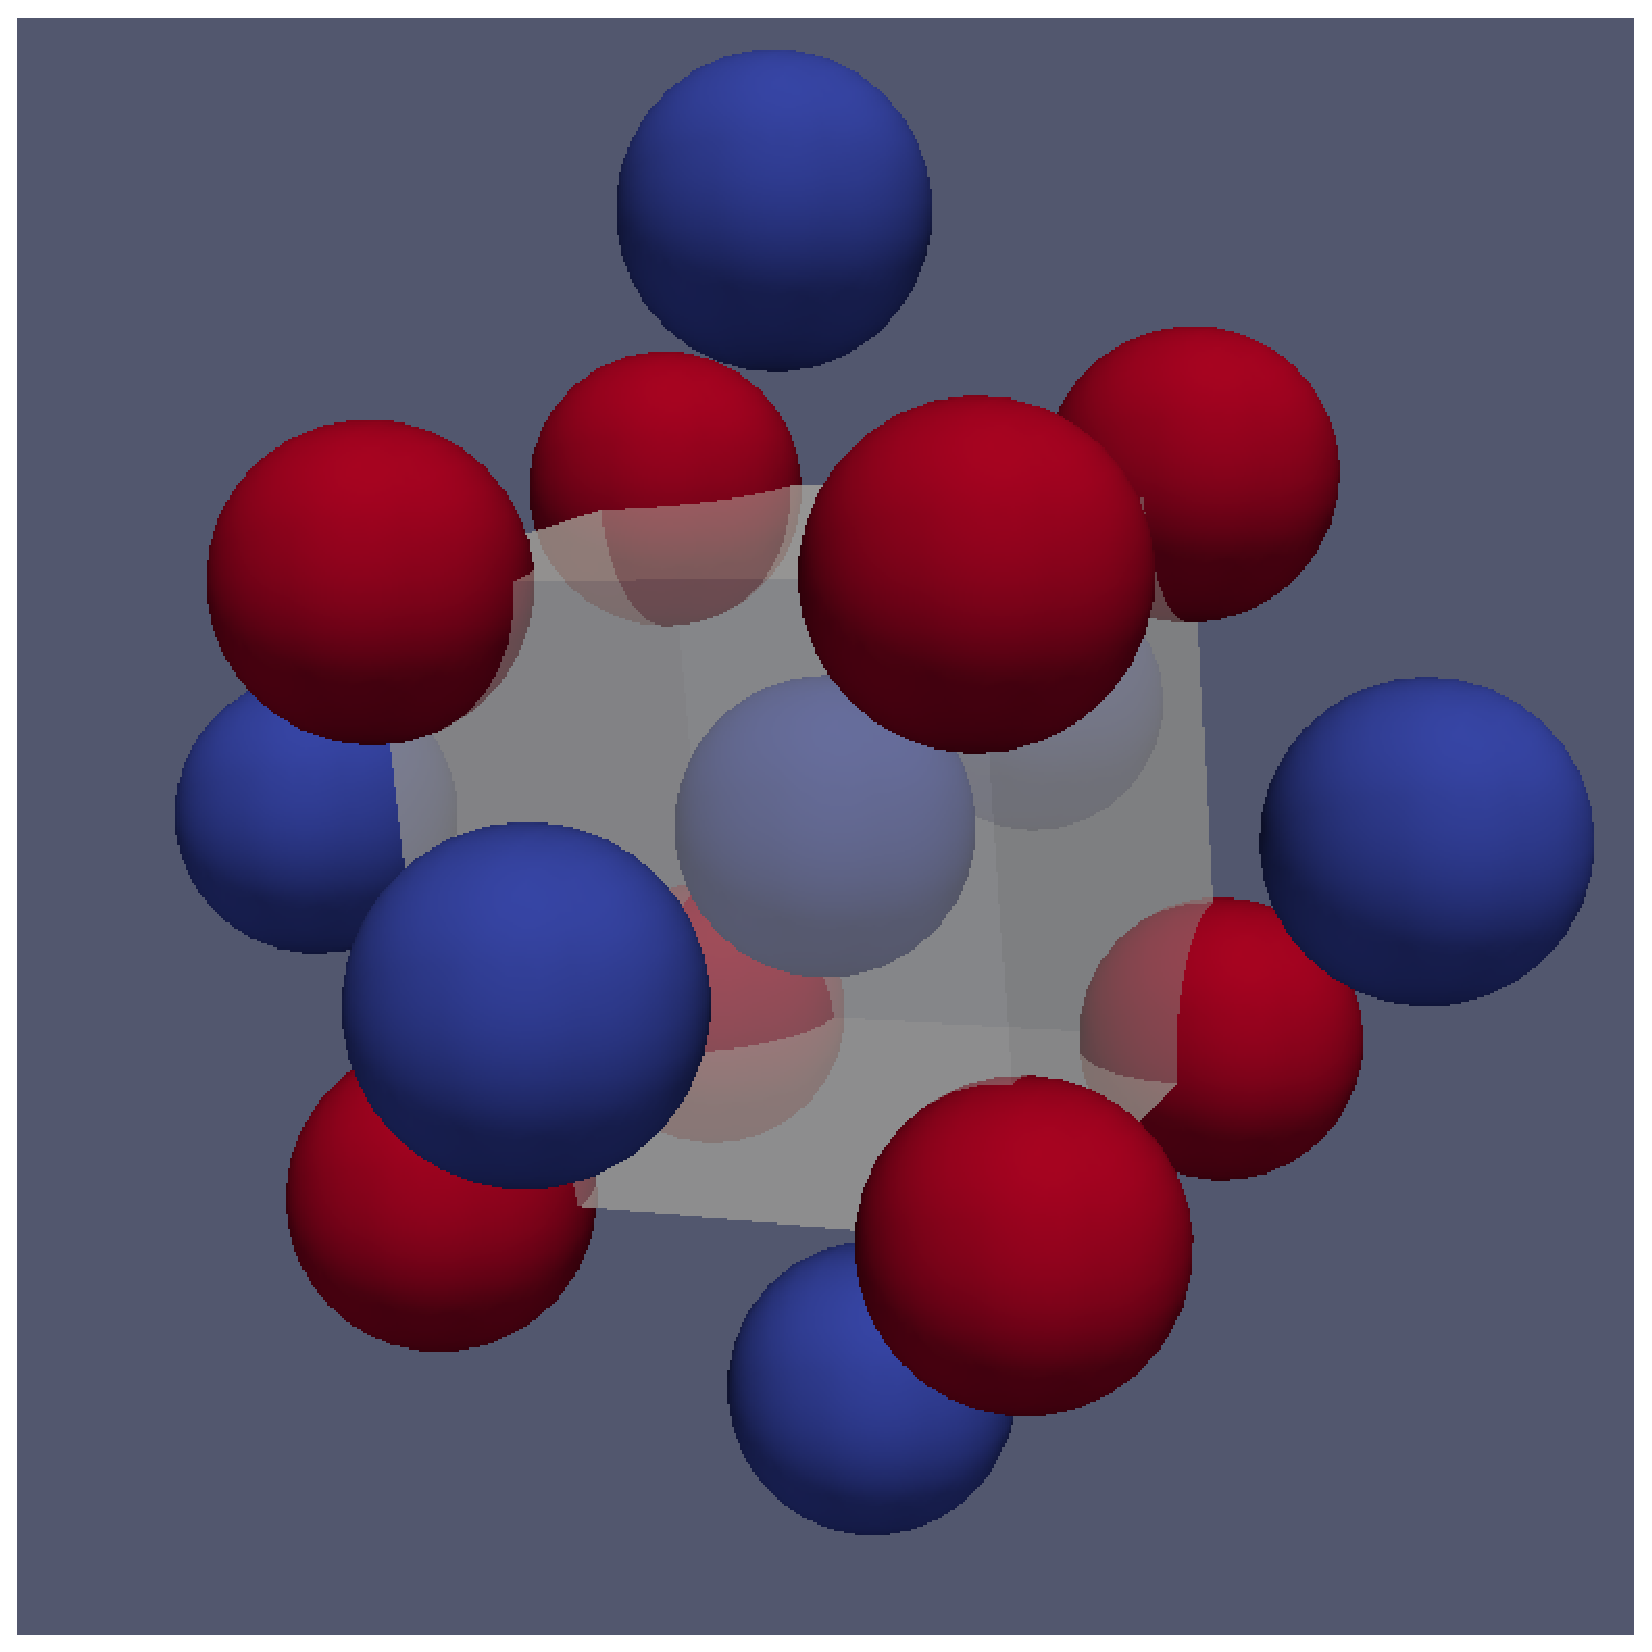
\includegraphics[width=0.25\columnwidth]{bcc_15}};
		\node[right=0 of bcc] (hcp) {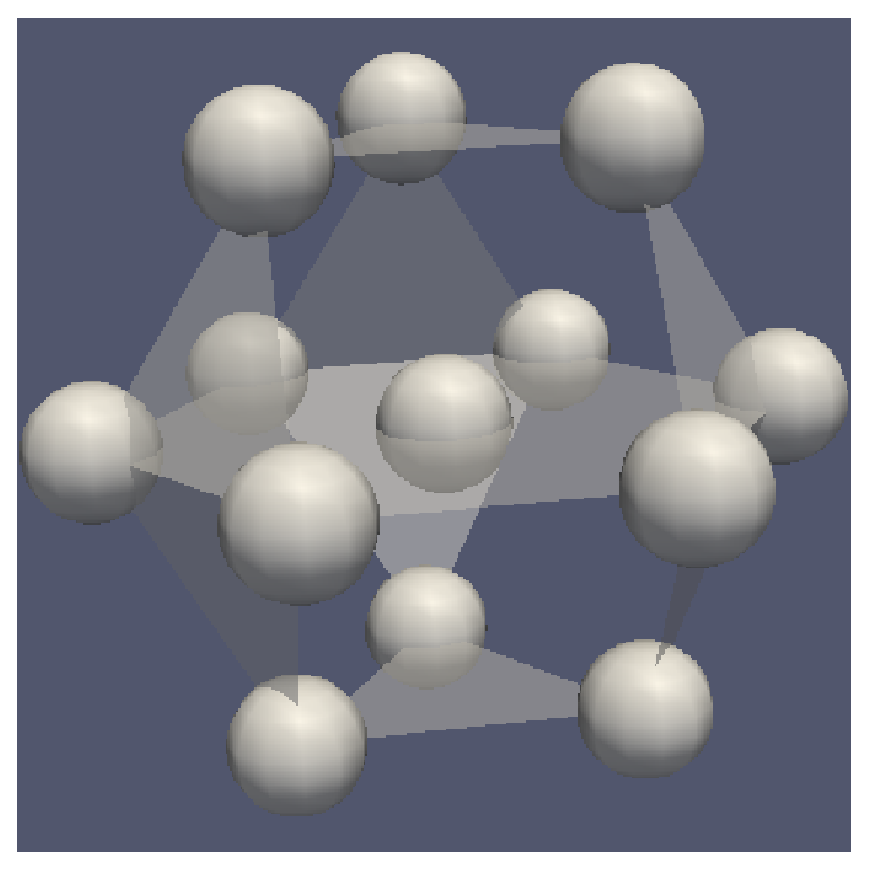
\includegraphics[width=0.25\columnwidth]{hcp_13}};
		\node[right=0 of hcp] (fcc) {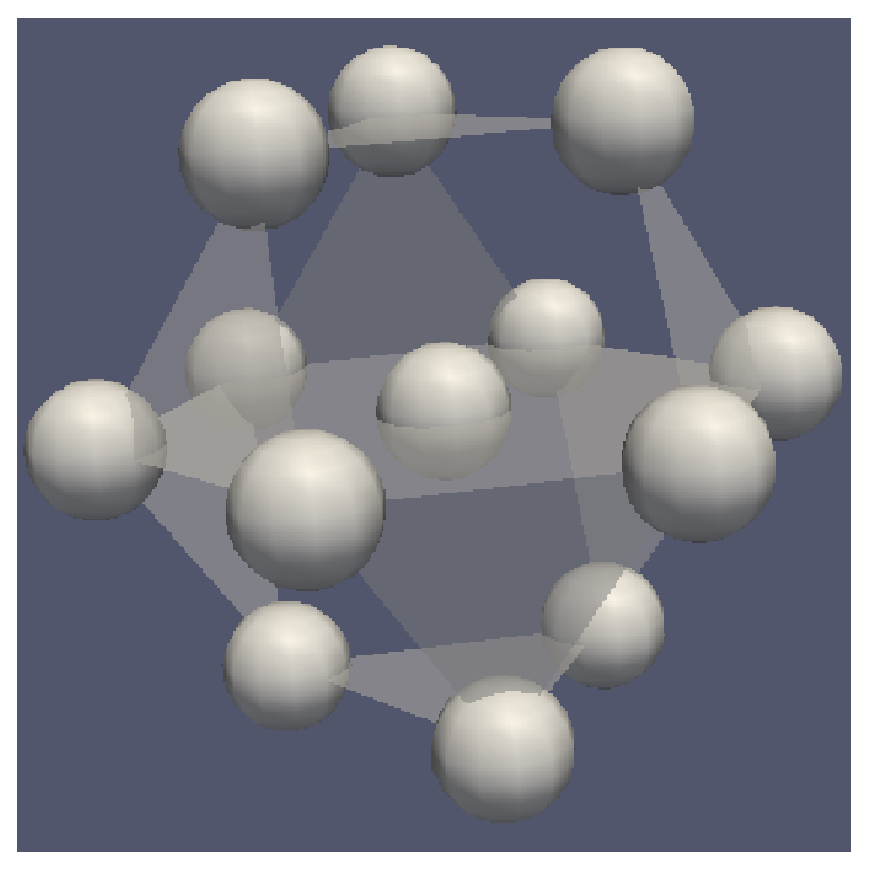
\includegraphics[width=0.25\columnwidth]{fcc_13}};
		\begin{axis}[%
			anchor=north east, at=(fcc.south east),%
			width=\columnwidth, height=\columnwidth,%
			ylabel={$Q_6$}, xlabel=$Q_4$,%
			xmin=0,xmax=0.22,%
			ymin=0, ymax=0.6,%
			enlargelimits=false,axis on top,
			extra tick style={grid=major},%
			extra y ticks={\Qstar}, extra y tick labels={},%
			xticklabel={$\pgfmathprintnumber[fixed,precision=2]{\tick}$}
			] 
		\alt<-2>{\addplot graphics
		[xmin=0,xmax=0.2,ymin=0,ymax=0.6]
		{lechner_Q4Q6.png};
		\matrix[
			matrix of nodes, ampersand replacement=\&, matrix anchor=south east,%
			nodes={inner sep=0.25em, anchor=west},%
			column 1/.style={circle},%
			] at (rel axis cs:1,0)
		{
			|[fill=black]| \& \textsc{bcc}\\
			|[fill=orange!80!black]| \& \textsc{fcc}\\
			|[fill=green!80!black]| \& \textsc{hcp}\\
			|[fill=blue!80!black]| \& aperiodic\\
		};
		}{\addplot graphics
		[xmin=0,xmax=0.2,ymin=0,ymax=0.6]{Q4Q6phi3954.png};}
		
		\node at (axis cs:0.1909, 0.5745) (infcc){};
		\node at (axis cs:0.0972222, 0.484762) (inhcp){};
		\node at (axis cs:0.0363696, 0.510688) (inbcc){};
		\end{axis}
		\draw[->, black] (bcc) -- (inbcc);
		\draw[->, green!80!black] (hcp) -- (inhcp);
		\draw[->, orange!80!black] (fcc) -- (infcc);
	\end{tikzpicture}
	\column{0.5\textwidth}
	\alt<1>{%
	{\footnotesize\citet{lechner2008}}

	\bigskip	
	
	\begin{itemize}
		\item $Q_\ell$ is the strength of the $\ell$-fold symmetry
		\item Very good at telling apart
			\begin{itemize}
				\item aperiodic structures
				\item locally periodic
			\end{itemize}
		\item Differentiate between crystal structures
	\end{itemize}
	
	\bigskip	
	%
	}{\tikzsetnextfilename{Q4Q6}
	\begin{tikzpicture}
		\begin{axis}[%
			width=\columnwidth, height=\columnwidth,%
			ylabel={$Q_6$}, xlabel=$Q_4$,%
			xmin=0,xmax=0.22,%
			ymin=0, ymax=0.6,%
			enlargelimits=false,axis on top,
			colormap={bw}{gray(0cm)=(1); gray(1cm)=(1); gray(10cm)=(0)},%
			colorbar sampled, colorbar horizontal, 
			colorbar style={%
				xlabel={per units of $Q_4\cdot Q_6$},% 
				xticklabels={$10^{1}$, $10^{2}$, $10^{3}$, $10^{4}$},%
				samples=6, xtick={ 0.20,0.4,0.6, 0.8},% 
				extra y ticks={},%
				/pgfplots/colorbar shift/.style={yshift=0.3cm},
				at={(parent axis.north)}, anchor=below south, width=0.9*\pgfkeysvalueof{/pgfplots/parent axis width},
				xticklabel pos=upper,%
				label style={font=\footnotesize},
				},%
			xticklabel={$\pgfmathprintnumber[fixed,precision=2]{\tick}$},%
			extra tick style={grid=major},%
			extra y ticks={\Qstar}, extra y tick labels={},%
			]
		\addplot graphics
		[xmin=0,xmax=0.2,ymin=0,ymax=0.6]
		{Q4Q6go1};
		\node [below] at (axis cs:0.1909, 0.5745) {\textsc{fcc}};
		\node [below] at (axis cs:0.0972222, 0.484762) {\textsc{hcp}};
		\node [below] at (axis cs:0.0363696, 0.510688) {\textsc{bcc}};
		\draw[->, white,thick] (axis cs:0.05, 0.15) to [out=60, in=220] (axis cs:0.125, 0.4);
		\end{axis}
	\end{tikzpicture}}
	\end{columns}
\end{frame}

\begin{frame}{Icosahedral order}
	\begin{textblock*}{0.6\textwidth}(10mm,88mm)
		\simplephasediagram{%
			\node at (0.576,0) [xp marker, fill=green!50!black] {};%
			\node at (0.497,0) [xp marker, fill=green!50!black] {};}
	\end{textblock*}
	\begin{columns}
	\column{0.5\textwidth}
	$w_6$
		\begin{itemize}
		\item first shell only
		\item sensitive to aperiodic
		\item icosahedral order stands out
		\end{itemize}
	\column{0.5\textwidth}
	\begin{block}{Two types of order}
		\begin{itemize}
		\item orthogonal
		\item incompatible
		\item mutual frustration
		\end{itemize}
	\end{block}
	\end{columns}
	\begin{center}\tikzsetnextfilename{w6Q6}
	\begin{tikzpicture}
		\pgfplotsset{
			extra tick style={grid=major},%
			every axis/.append style={%
				height=0.4\textwidth,
				ymin=0,ymax=0.6,%
				extra y ticks={\Qstar}, extra y tick labels={},%
				enlargelimits=false,axis on top,
				colormap={bw}{gray(0cm)=(1); gray(1cm)=(1); gray(10cm)=(0)},%
				colorbar sampled,%
				},%
		}
		\begin{groupplot}[
			group style={
				group size=2 by 1,%
				yticklabels at=edge left,%
				horizontal sep=0pt,%
				},%
			anchor=above north west,%
			width=0.38\textwidth,%
			xlabel=$10^2 \cdot w_6$,%
			xmin=-0.052,xmax=0.01,%
			extra x ticks={\wstar, -0.00782},%
			extra x tick labels={,},%
			xtick scale label code/.code={},%
			colorbar right, colorbar style={%
				samples=6, ytick={ 0.20,0.4,0.6, 0.8},% 
				yticklabels={$10^{1}$, $10^{2}$, $10^{3}$, $10^{4}$},%
				ylabel={per units of $w_6\cdot Q_6$},%
				extra x ticks={},%
				extra y ticks={},%
				label style={font=\footnotesize},
				},%
			]
		\nextgroupplot[ylabel={$Q_6$}, xtickmax=0,]
		\addplot graphics
		[xmin=-0.052,xmax=0.052,ymin=0,ymax=0.6]
		{u6Q6phi3954_scale};
		\node [above] at (axis cs:-0.04, \Qstar) {\footnotesize{$Q_6^*$}};
		%\node [anchor=north east] at (rel axis cs:1, 1) {\footnotesize{$\phi = 0.497 \pm 0.03$}};
		\node [left] at (axis cs:\wstar,0.4) {\footnotesize $w_6^*$};
		\node [right] at (axis cs:-0.00782,0.4) {\footnotesize $w_6^{dod}$};
		
		\nextgroupplot
		\addplot graphics
		[xmin=-0.052,xmax=0.052,ymin=0,ymax=0.6]
		{u6Q6go1_scale};
		\node at (axis cs:\wstar,0.6) (a) {};
		\node at (axis cs:-0.00782,0.6) (b) {};
		\node [below] at (axis cs:-0.0026, 0.5745) {\textsc{fcc}};
		\node [below, right] at (axis cs:-0.052, 0.05) {\textsc{Ico}};
		\draw[->, white,thick] (axis cs:-0.001, 0.15) to [out=90, in=275] (axis cs:-0.0015, 0.33);
		\draw[->, white,thick] (axis cs:-0.001, 0.15) to [out=180, in=30] (axis cs:-0.025, 0.12);
		
		\end{groupplot}
	\end{tikzpicture}\end{center}
\end{frame}